\documentclass[a4paper,12pkt]{report}
\usepackage[utf8]{inputenc} %Specialtegn
\usepackage{amsmath} %Matricer og Mat symboler
\usepackage{graphicx} %Billeder og Figurer
\usepackage{setspace} %Mellemrum mellem linjer og paragraffer
\usepackage{amssymb} %Mat symboler
\usepackage[danish]{babel} %Stavekontrol
\usepackage{fancyhdr} %Headers
\usepackage{csquotes} %Citeringer over flere dokumenter
\usepackage[a4paper, total={6in, 8in}]{geometry} %Bredere Marginer
\usepackage[backend=biber]{biblatex} %Gør det muligt at have litteraturliste med flere subfiles
\addbibresource{Litteratur.bib} %Litteraturliste
\bibliography{Litteratur.bib} %Litteraturliste
\usepackage[colorlinks]{hyperref} %Hyperlinks i PDF
\title{Scienfic Computing Project 1 }
\author{Anders Kjølhede}
\date{September 2022}

\begin{document}

\pagestyle{fancy}
\fancyhf{}
\rhead{Scienfic Computing}
\lhead{nr.1}
\rfoot{side \thepage}

\maketitle

\onehalfspacing %Linjeafstand
\setlength{\jot}{10pt} %Mellemrum ved ligninger

\section*{Background Theory}

The polarizability for a given frequency $\omega$ is obtained as a scalar product of two vectors \textbf{z} and \textbf{x}.

\begin{equation}
    \alpha(\omega) = z^Tx
\end{equation}

\textbf{z} is obtained from the schrödinger equation and \textbf{x} is the solution to the following system of linear equation:

\begin{equation}
    (E-\omega S)x = z
\end{equation}

E and S are square matrices and $\omega$ is the frequency of the incoming light. E, S and z are visualized as follows:

\begin{equation}
    E = \begin{bmatrix}
        A & B \\
        B & A
    \end{bmatrix}
    \hspace{1cm}
    S = \begin{bmatrix}
        I & 0 \\
        0 & -I
    \end{bmatrix}
    \hspace{1cm}
    z = \begin{bmatrix}
        y \\
        -y
    \end{bmatrix}
\end{equation}

\section*{Question A}

By computing the max-norm and the inverse of the given matrix we can calculate the condition number for the individual frequencies by using the following relation:

\begin{equation}
    cond_{\infty}(M) = ||M||_{\infty}||M^{-1}||_{\infty}
\end{equation}



\begin{table}[h!]
    \centering
    \begin{tabular}{l  c  c  c }
    \hline
     Frequencies & Condition Number & Sig. digits \\ \hline
     0.800 & 327.8167 & 5\\
     1.146 & 152679.2687 & 2\\
     1.400 & 227.1944 & 5
    \end{tabular}
    \caption{}
    \label{Confusion matrix scores}
\end{table}

\section*{Question B}

For the three frequencies we can also determine a bound on the relative forward error in the max-norm:

\begin{equation}
    \frac{||\delta x||_{\infty}}{||\hat{x}||_{\infty}} \leq cond_{\infty}(E-\omega S) \frac{||\delta \omega S||_{\infty}}{||E-\omega S||_{\infty}}
\end{equation}

The values for this is shown in tabel 2 

\begin{table}[h!]
    \centering
    \begin{tabular}{l  c  c  c }
    \hline
     Frequencies & Bound & Sig. digits\\ \hline
     0.800 & 0.0052 & 2 \\
     1.146 & 2.4050 & 0 \\
     1.400 & 0.0035 & 2
    \end{tabular}
    \caption{}
\end{table}

$\omega$ is given with three significant digits and by taking the negative logarithm to the relative error we can calculate the amount of significant digits in x.

\newpage

\section*{Question C}

I have implemented three functions for calculating the forward and backward substitution, and at last LU factorization. These have been tested against a library routine and succesfully got the same result for the linear system in eq. 6


\begin{equation}
    \begin{bmatrix}
        2 & 1 & 1\\
        4 & 1 & 4 \\
        -6 & -5 & 3
    \end{bmatrix}
    \begin{bmatrix}
        x_1  \\
        x_2 \\
        x_3
    \end{bmatrix}
    =\begin{bmatrix}
        4 \\
        11 \\
        4
    \end{bmatrix}
\end{equation}

The solution to this system of equations is shown below

\begin{equation}
    \begin{bmatrix}
        x_1 \\
        x_2 \\
        x_3 
    \end{bmatrix} = 
    \begin{bmatrix}
        -4 \\
        7 \\
        5 
    \end{bmatrix}
\end{equation}

\section*{Question D}

We now want to calculate the frequency dependent polarizability using our routines from Question C and the frequencies along with their pertubations $\omega \pm \delta$. The results are shown in table 4.

\begin{table}[h!]
    \centering
    \begin{tabular}{l  c  c  c }
    \hline
     Frequencies & $a(\omega)$ & $a(\omega+\delta)$ & $a(\omega-\delta)$ \\ \hline
     0.800 & 1.636 & 1.644 & 1.627\\
     1.146 & 2604 & -4185 & 994.8\\
     1.400 & -2.708 & -2.699 & -2.713
    \end{tabular}
    \caption{}
\end{table}

The variation is due to a pertubation in $\omega$ and this is part of the matrix $(E-\omega S)$ and if we assume z to be exact then the (b) bound is correct.

\section*{Question E}

We now want to see if we calculate $a(\omega)$ for all values in the interval $[0.7,1.5]$.

\begin{figure}[h]
    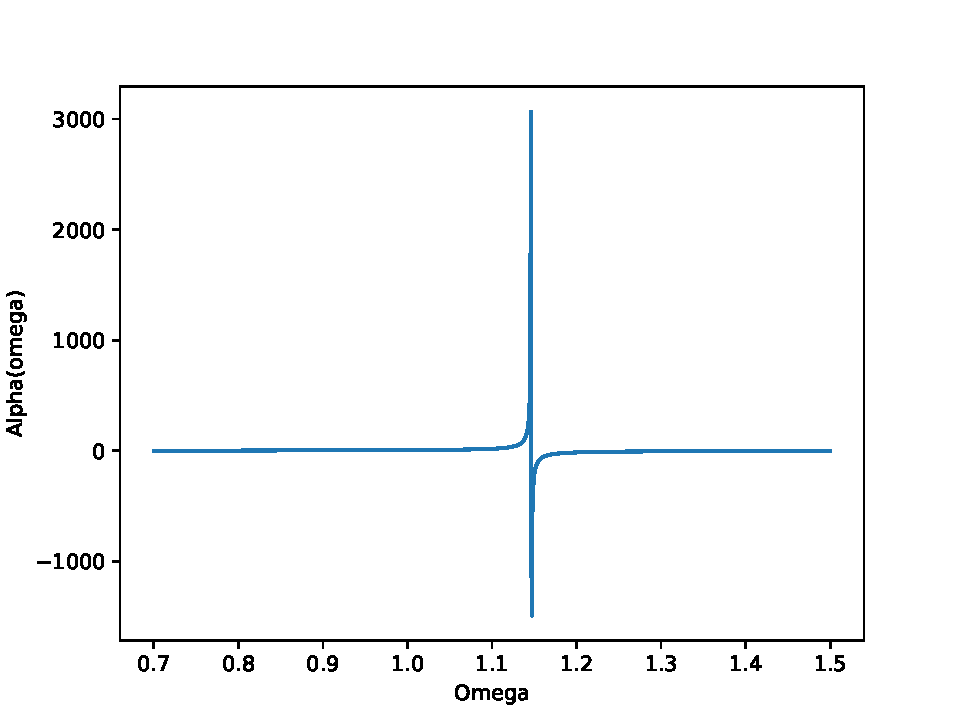
\includegraphics[width = 12cm]{e1.pdf}
    \centering
\end{figure}

\noindent
At $\omega = 1.146307999$ the polarizability approaches a non-singularity and we saw that the condition number for this specific value of $\omega$ was very high, see table 1


\section*{Question F}

\textbf{F1}: We now want to implement and test other means of solving linear systems than the previously used LU factorization. For this we can introduce QR factorization and linear least squares. The QR factorization takes a rectangular matrix M and return two square matrices in the form of Q and R. We can check that the solution is correct by verifying that $Q^TQ=QQ^T=I$ and $M = QR$

\noindent
\textbf{F2}: I tried to implement a faster householder algorithm but this unfortunately gave the wrong R matrix.

\noindent
\textbf{F3}: The least squares routine can be testet against A2 and B2 from HHexamples.py. This yields the same result as the libeary routine from np.lialg.

\begin{equation}
    \begin{bmatrix}
        x_1 \\
        x_2 \\
        x_3 
    \end{bmatrix} = 
    \begin{bmatrix}
        -4 \\
        7 \\
        5 
    \end{bmatrix}
\end{equation}




\section*{Question G}

\textbf{G1}: Due to severe discontinuity in $\omega = 1.146307999$ i have chosen a cut off point at $1.1$.

\noindent
\textbf{G2}: Solution can be seen in .py file

\noindent
\textbf{G3}: Solution is plottet in fig. 2 and one can see that the relative error is smaller for the polynomial $n = 6$

\begin{figure}[h]
    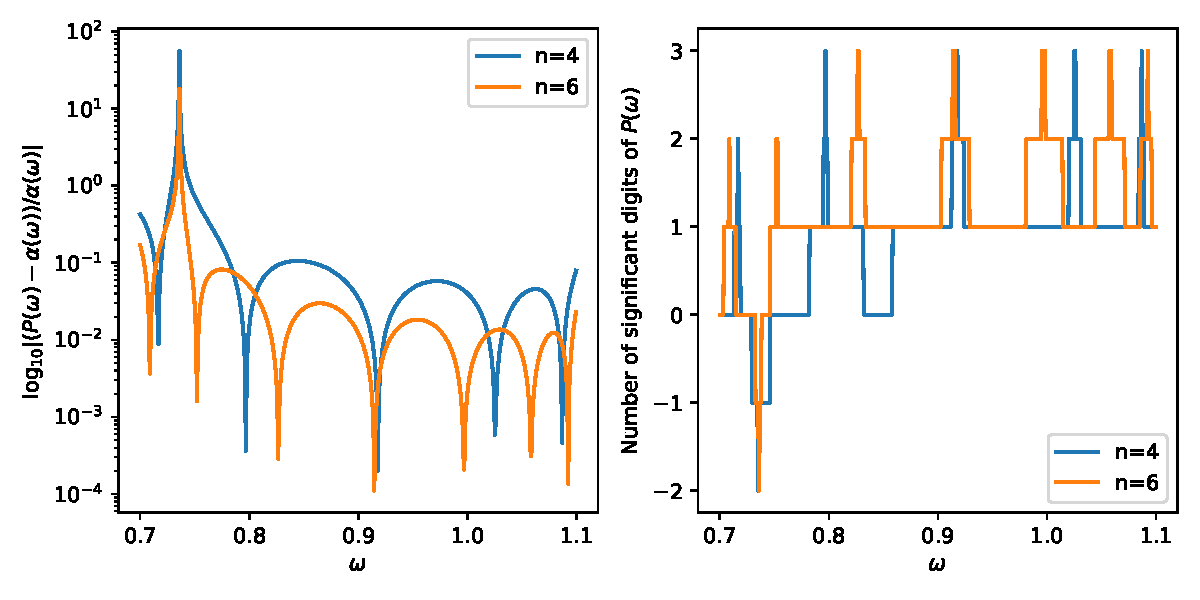
\includegraphics[width = 12cm]{g.pdf}
    \centering
\end{figure}

\noindent
\textbf{G4}: The number of significant digits depends on which value of $\omega$ we choose to look at, but generally one can see that the polynomial $n = 6$ gives a better result

\section*{Question H}

\noindent
\textbf{H1}: Could not work this one out.



\noindent
\textbf{H2}: We can calculate the a and b coefficients using our implemented least squares routine and using this to calculate the Q approximation. 
These two approximations for $n=2$ and $n=4$ are shown in fig 3. along with ther respective significant digits for each $\omega$.



\noindent
\textbf{H3}: I did not have time to complete this one.


\begin{figure}[h]
    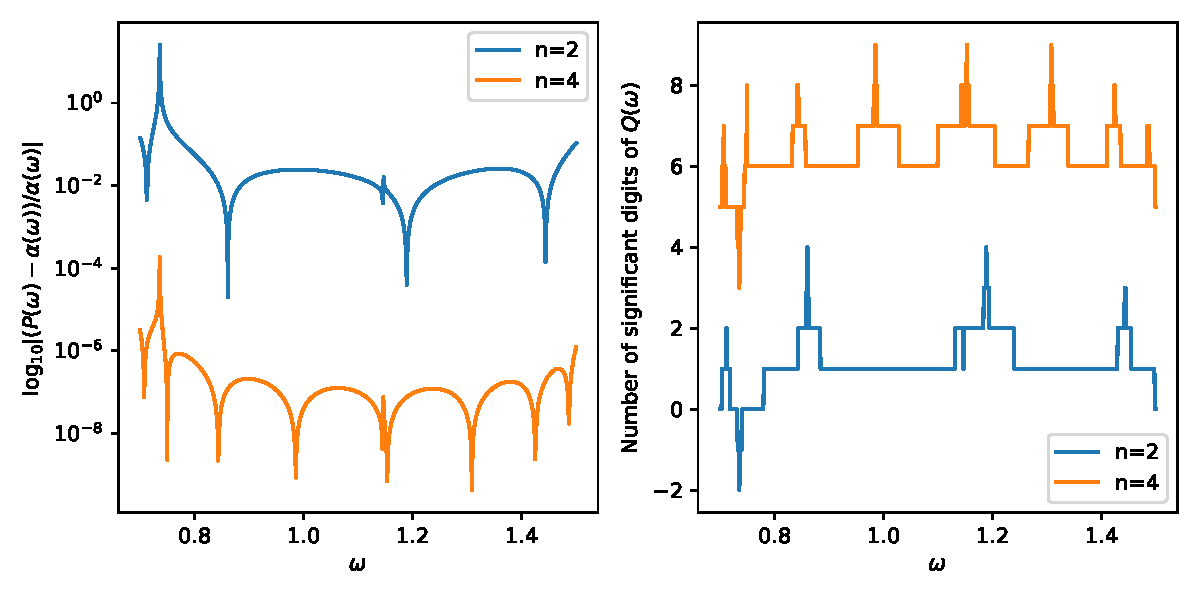
\includegraphics[width = 12cm]{h.pdf}
    \centering
\end{figure}

\end{document}